\RequirePackage[l2tabu, orthodox]{nag} % Warn about outdated commands/packages.
% The report class uses some outdated commands, about which nag will complain.
% You can just ignore these warnings.

\documentclass[11pt, a4paper]{report} % Sets font and paper size.

%%% General formatting packages (order is important, so don't sort) %%%
\usepackage{amsmath} % More equation formatting.
\usepackage{amssymb}
\usepackage{amsthm}
\usepackage[english]{babel} % Language specific quirks.
\usepackage{cite}
\usepackage{epigraph}
\usepackage{booktabs} % Improved tables.
\usepackage[font=small]{caption} % Better caption formatting.
\usepackage{fancyhdr} % Modification of headers and footers.
\usepackage[T1]{fontenc} % Makes one unicode character of special input (e.g. ö).
\usepackage[margin=1.25in]{geometry} % Control page layout.
\usepackage{float} % More control over image positions.
\usepackage{graphicx} % Include graphics. Use '\graphicspath' to locate files in a different folder.
\usepackage[utf8]{inputenc} % Special characters (e.g. trema) can be entered directly: .tex file has to be saved using UTF-8 encoding.
\usepackage{lmodern} % Alternative font because 'fontenc' package does not work with default.
\usepackage{microtype} % Improves character spacing.
\usepackage{physics} % Provides physics macros such as Dirac notation.
\usepackage{tikz} % Draw diagrams and figures.
\usepackage{url} % Allow inclusion of urls in text.
\usepackage{siunitx} % SI unit formatting and scientific notation.
\usepackage{subcaption} % Allow subcaptions.
\usepackage[nottoc]{tocbibind} % Include references in table of contents.
\usepackage[colorinlistoftodos,textsize=tiny]{todonotes} % Add todo notes.
\usepackage{hyperref}
\usepackage[noabbrev]{cleveref} % Automate "equation (...)" reference. Use \cref.
\usepackage{doi}

\hypersetup{colorlinks, citecolor=blue, filecolor=black, linkcolor=blue, urlcolor=blue } 



%%% Additional options %%%
\pagestyle{fancy} % Set header style.
\fancyhead[L]{\rightmark}
\fancyhead[R]{}
\setlength{\headheight}{14pt}

\setcounter{tocdepth}{10}
\setcounter{secnumdepth}{10}
\setcounter{MaxMatrixCols}{20}


%%% Personal Information %%%
\newcommand\TITLE{Summing matrix elements of the Lieb-Liniger model with reinforcement learning\\}
\newcommand\THESISFORM{Master Thesis}
\newcommand\AUTHOR{Teun Zwart}
\newcommand\SUPERVISOR{Prof. dr. Jean-Sébastien Caux}
\newcommand\SECONDASSESSOR{dr. Jasper van Wezel}
\newcommand\UNIVERSITYLOGO{} % Uncomment line below and add name of logo file.

\newcommand{\bea}{\begin{align}}
\newcommand{\ena}{\end{align}}

\newcommand{\inversetruncc}{\mathcal{L}}
\newcommand{\kernel}{\mathcal{C}}
\newcommand{\operator}{\mathcal{O}}

% Prevent all line breaks in inline equations.
\binoppenalty=10000
\relpenalty=10000

\newtheorem{theorem}{Theorem}


\begin{document}

\begin{titlepage}
	\begin{center}
		% \includegraphics[width=\textwidth]{\UNIVERSITYLOGO}
		\rule{\textwidth}{0.4mm}\\[0.5cm]
		\huge{\textbf{\TITLE}}
		\rule{\textwidth}{0.4mm}\\[0.5cm]
		\Large{\THESISFORM}\\[0.5cm]
		\begin{minipage}[t]{0.4\textwidth}
			\begin{flushleft}
				\large\emph{Author:}\\{\AUTHOR}
			\end{flushleft}
		\end{minipage}
		\begin{minipage}[t]{0.4\textwidth}
			\begin{flushright}
				\large\emph{Supervisor}\\{\SUPERVISOR}\\~\\
				\large\emph{Second Assessor}\\{\SECONDASSESSOR}\\~\\~\\
			\end{flushright}
		\end{minipage}
		\vfill
		\large \today\\
	\end{center}
\end{titlepage}

\newpage
\thispagestyle{empty}

\ 
\vspace{4cm}

\epigraph{\itshape Science is just magic that works.}{Kurt Vonnegut}

\epigraph{\itshape All sufficiently advanced technology is indistinguishable from magic.}{Arthur C. Clark}


\tableofcontents

\section*{TODO}
\begin{itemize}
  \item \url{http://ataspinar.com/2017/08/15/building-convolutional-neural-networks-with-tensorflow/}
  \item interesting for presentation \url{https://www.alexirpan.com/2018/02/14/rl-hard.html}
\end{itemize}

\newpage

\section*{Abstract}

\chapter{Introduction}

\epigraph{\itshape The future is already here -- it's just not very evenly distributed.}{William Gibson}

Currently, in the ABACUS algorithm, dynamic structure factors for various Bethe-ansatz integrable models are calculated.
This is done by summing over intermediate states to get the Lehmann series representation of the Fourier transform of the DSF.

The order of summation determines how quickly saturation of the f-sum rule occurs.
To maximize efficiency we only want to sum those state that contribute significantly to the DSF.
This may be done by efficiently scanning through the state space of the model.
There is an optimum way to do this, but it is not clear what this is.
Currently heuristics are used to select states.
This is already efficient since only very small fractions of the state space are used to reach saturations in excess of 99\%.
However, a more efficient summation is still desirable.

In this work we consider reinforcement learning as a way to sum the state space in an efficient way.
Inspired by computers playing both 1980's video games \cite{mnih13_playin_atari_with_deep_reinf_learn} and recent advances in machine learning approaches to the board game Go\cite{Silver2017a,Silver2017}, we create a neural network that can efficiently determine which states are the most promising to sum when scanning the state space of a model.

This may also generalize to models beyond the Lieb-Liniger model.
Since the scanning is model independent (only taking in the Bethe numbers of the model), as long as the f-sum rule for the desired DSF is known, we can optimize the state scanning.

It is also possible that transfer learning may be used to map the experience gained in smaller systems to larger systems.
This may be done with either convuloutional downsampling or restricted Boltzmann machines.

This thesis is laid out as follows:
in \cref{chap:bethe_ansatz} we review some of the basics of the Bethe ansatz and its application in the Lieb-Liniger model.
\Cref{chap:abacus} describes the ABACUS algorithm; its use and current implementation of the state scanning algorithm.
In \cref{chap:machine_learning} an introduction to machine learning and specifically reinforcement learning is given.
We describe our approach and results in \cref{chap:results}.
Finally \cref{chap:conclusion} summarizes our results and makes recommendations for future research directions.




\begin{itemize}
  \item \textbf{How can we efficiently scan through the state space of the Lieb-Liniger model?}
  \item How does ABACUS currently do this?
  \item Is this approach amenable to machine learning? (Specifically reinforcement learning through minimization of the number of summed states necessary to reach a given f-sum rule saturation)
  \item Would transfer learning allow the result of this to be maped to different system sizes (through convolutional down sampling/ restricted Boltzman machines)
  \item What would be the nbest neural network approach be to deicde on the next best state to sum? \\ How do we choose? The number of edges grows linarly in time, making it difficult to have aprobability ditribution over them. We also have to keep in mind the constraints on the Bethe numbers of the Lieb-Liniger model.    
  \item How do we backpropagate the succes/failure of a run through the network (see ALPHA GO)?
  \item Does this generalize to other models? It should, as long as you are able to find the DSF's you are interested in since you need them for the sum rule.
  \item Would an RNN scanning over the history of the summation work better?
  \item Control: How does random sampling of the space perform in f-sum rule summation?
  \item
  \item How does a neural net perform on predicting rapidities and matrix elements?
\end{itemize}

\chapter{The Bethe Ansatz}\label{chap:bethe_ansatz}

The Bethe Ansatz allows for a way to solve certain one-dimensional systems exactly.
It was put forth by Bethe in 1931 to solve the Heisenberg model, refining and correcting the earlier work of Bloch \cite{Bethe1931}.

\section{The Lieb-Liniger model}

Here, to introduce and understand the Bethe Ansatz, we focus on the Lieb-Liniger model, finding its eigenfunctions and excitation spectrum.
The Lieb-Liniger model, first introduced by Lieb and Liniger in 1963 \cite{Lieb1963, Lieb1963a}, consists of bosons interacting through a delta-function potential, described by the Hamiltonian
\begin{equation}
	H = - \sum_{j=1}^{N} \frac{\partial^2}{\partial x_j^2} + 2c \sum_{j<l} \delta(x_j - x_l).
\end{equation}
Here \(c\) is the interaction strength of the model, \(\hbar=1\) and we set \(2m=1\).
In the limit \(c\to0\) particles behave as free bosons, while \(c\to\infty\) yields fermionic behaviour and is known as the Tonks-Girardeau model \cite{Lieb1963, Franchini2017}.

We will only solve the repulsive case (\(c > 0\)) here.

\subsection{A solution for the Schrödinger equation}

We will start solving the Lieb-Liniger model in the two-particle case. This later readily generalizes to many particles.

For two particles, the Hamiltonian becomes
\begin{equation}
	H =  - \frac{\partial^2}{\partial x_1^2} - \frac{\partial^2}{\partial x_2^2} + 2c \delta(x_1 - x_2).
\end{equation}
We can write this in a more convenient form without the delta-function by integrating the Schrödinger equation over a small interfal \([-\epsilon,\epsilon]\).
This yields the condition \cite{Lieb1963}\todo{Do this explicitly.}\footnote{This operation is relatively simple but does contain a few subtleties. Let us therefore do it explicitly:
the Schrödinger equation is
\begin{equation}
	\left[- \frac{\partial^2}{\partial x_1^2} - \frac{\partial^2}{\partial x_2^2} + 2c \delta(x_1 - x_2)\right] \psi(x_1, x_2) = E \psi(x_1,x_2).
\end{equation} 
Integrating \cite{Griffiths1993}
}
\begin{equation}\label{eq:lieblinigerboundary}
	\left[\frac{\partial}{\partial x_2} - \frac{\partial}{\partial x_1} - c\right] \psi(x_1, x_2)\bigg\rvert_{x_1 = x_2} = 0.
\end{equation}
Since particles only interact with each other when their positions coincide, this allows us to simplify the Schrödinger equation to
\begin{equation}\label{eq:lieblinigersimple}
	\left[- \frac{\partial^2}{\partial x_1^2} - \frac{\partial^2}{\partial x_2^2}\right] \psi(x_1, x_2) = E \psi(x_1,x_2),
\end{equation}
with \cref{eq:lieblinigerboundary} as a boundary condition \cite{Lieb1963}.
Since we are dealing with bosons, we also require the wavefunction to be symmetric: \(\psi(x_1,x_2) = \psi(x_2,x_1)\).
Effectively we have rewritten the Schrödinger equation such that we only consider the wave function away from the delta-function interaction points.
The boundary condition then reintroduces the interaction terms.
We also assume an ordering of the positions \(x_1 < x_2\).

We can now conjecture a solution for the Lieb-Liniger model based on \cref{eq:lieblinigersimple}.
This equation can be solved in terms of a superposition of plane waves:
\begin{equation}
	\psi(x_1,x_2) = A_{12} e^{i(\lambda_1x_1 + \lambda_2 x_2)} + A_{21} e^{i(\lambda_2 x_1 + \lambda_1 x_2)},
\end{equation}
where the \(\lambda\)'s are pseudo-momenta, so-called because they are unobservable \cite{Franchini2017}.
The \(A\)'s are the amplitudes of the planewaves making up the wavefunction.
Since \cref{eq:lieblinigerboundary} has to be fulfilled we require the amplitudes be related to each other by
\begin{align}
	\frac{A_{12}}{A_{21}} = -\frac{c-i(\lambda_1 - \lambda_2) }{c+i(\lambda_1 - \lambda_2)}.
\end{align}
The right-hand side of this equation has modulus 1, meaning it can be written as a phase:
\begin{align}
	\frac{A_{12}}{A_{21}} = -e^{i\phi(\lambda_1-\lambda_2)},
\end{align}
where \cite{Korepin1993}
\begin{align}
  \phi(\lambda_1-\lambda_2) = i \log(\frac{\lambda_1-\lambda_2 + ic}{\lambda_1-\lambda_2-ic})
\end{align}
or
\begin{align}
	\phi(\lambda_1-\lambda_2) = -2\arctan\left(\frac{\lambda_1-\lambda_2}{c}\right),
\end{align}
if we assume the argument of \(\phi\) to be real \cite{Lieb1963}.

We can now write the two-particle wavefunction by setting \(A_{21}=1\) (and ignoring normalization for the moment) to get
\begin{equation}
	\psi(x_1,x_2) = - e^{-\frac{i}{2}\phi(\lambda_1-\lambda_2)+i(\lambda_1x_1 + \lambda_2 x_2)} + e^{\frac{i}{2}\phi(\lambda_1-\lambda_2)+i(\lambda_2 x_1 + \lambda_1 x_2)}.
\end{equation}
Generalization to the whole domain (not just where \(x_1 < x_2\)) can be achieved by requiring the wavefunction to be fully symmetric under coordinate exchange,
yielding
\begin{equation}
  \psi(x_1,x_2) = \textrm{sgn}(x_2-x_1)\sum_{P\in\pi_2} (-1)^{[P]} e^{i\lambda_{P_1}x_1 + i \lambda_2 x_2- \frac{i}{2} \textrm{sgn}(x_2-x_1)\phi(\lambda_{P_1}-\lambda_{P_2})}.
\end{equation}
The sum runs over the permutations of the set \((1,2)\).
This wave function is antisymmetric under exchange of quasimomenta, meaning that any wave function in which \(\lambda_1=\lambda_2\) is equal to 0.
This points to a Pauli principle like phenomenon \cite{tofind}.


Going to the many-particle state is now a fairly straightforward generalization of the two-particle case.
The wavefunction in this case becomes \cite{Franchini2017}\todo{Bring the presentation of this in line with the two particle case.}
\begin{equation}
	\psi(x_1,\ldots,x_N) = \sum_{\mathcal{P}} A(\mathcal{P}) e^{i\sum_j \lambda_{\mathcal{P}_j} x_j}.
\end{equation}


\subsubsection{Quantization}

Since we would like to study the thermodynamics of the system, it is convenient to confine the system to a finite length \(L\).
This translates into a periodicity requirement for the wave function.
For two particles this means
\begin{align}
	\psi(x_1+L,x_2|\lambda_1,\lambda_2) = \psi(x_1,x_2+L|\lambda_1,\lambda_2) = \psi(x_1,x_2|\lambda_1,\lambda_2).
\end{align}
Imposing this condition on the wave function yields
\begin{align}
  e^{i\lambda_1L} = - e^{-i\phi(\lambda_1 - \lambda2)}, \qquad e^{i\lambda_2L} = - e^{i\phi(\lambda_1 - \lambda2)},
\end{align}
or explicitly \cite{tofind}
\begin{align}
  e^{i\lambda_1L} = \frac{\lambda_1-\lambda_2 + ic}{\lambda_1-\lambda_2-ic}, \qquad e^{i\lambda_2L} = \frac{\lambda_2-\lambda_1 + ic}{\lambda_2-\lambda_1-ic}.
\end{align}

These are known as the Bethe equations.
In logarithmic form this becomes 
\begin{align}\label{eq:bethe_equations}
  \lambda_1 + \frac{1}{L} \phi(\lambda_1-\lambda_2) = \frac{2\pi}{L} I_1, \qquad \lambda_2 + \frac{1}{L} \phi(\lambda_2-\lambda_1) = \frac{2\pi}{L} I_2.
\end{align}
The numbers \(I_1, I_2\) uniquelly label the quasimomenta and are hald-odd integers. 
They act as the quantum numbers of the theory \cite{tofind}.

In the many particle case the bethe equations generalise to
\begin{equation}
  e^{i\lambda_jL} = \prod_{l\neq j} \frac{\lambda_j-\lambda_l + ic}{\lambda_j - \lambda_l - ic}
\end{equation}
or in logarithmic form
\begin{align}
  \lambda_j + \frac{1}{L} \sum_{l=1}^N \phi(\lambda_j - \lambda_l) = \frac{2\pi}{L}I_j, \qquad j = 1,\ldots,N,
\end{align}
where \cite{tofind}
\begin{align}
I_j \in 
\begin{cases}
  \mathbb{Z} + \frac{1}{2}, \qquad &N \textrm{ even}\\
  \mathbb{Z}  &N \textrm{ odd}
\end{cases}
\end{align}

The Bethe equations and Bethe numbers have a number of different properties:

\begin{theorem}\label{th:convexity}
\begin{sloppypar}
\noindent
The solutions of the Bethe equations \cref{eq:bethe_equations} are unique and exist, given a \mbox{(half-)integer} set of quantum numbers \(\{I\}\) \textup{\cite{Yang1969}}.
\end{sloppypar}
\end{theorem}
\begin{proof}
This can be proven with a variational argument, where the Bethe equations are the extremum of an action.
The Yang-Yang action for the Lieb-Liniger model is
\begin{align}
	S= \frac{L}{2} \sum_{j=1}^{N} \lambda_j^2 - 2\pi\sum_{j=1}^{N} n_j \lambda_j + \frac{1}{2} \sum_{j=1}^N \sum_{k=1}^{N} \theta_1(\lambda_j - \lambda_k),
\end{align}
where \(\theta_1(\lambda) = \int_0^{\lambda} \theta(\mu)\dd\mu\).
The Bethe equations follow from this by setting \(\frac{\partial S}{\partial \lambda_j} = 0\), which corresponds to a minimum.
To show this we need to have a positive definite matrix of second derivatives:
\begin{align}
	\frac{\partial^2S}{\partial\lambda_j\partial\lambda_l} = \delta_{jl} \left[L + \sum_{m=1}^{N} K(\lambda_j,\lambda_m)\right] - K(\lambda_j, \lambda_l),
\end{align}
where 
\begin{align}
	K(\lambda, \mu) = \frac{2c}{c^2 + (\lambda - \mu)^2}.
\end{align}

Introducing a vector \(v_j\) with real components we get~\cite{Korepin1993}
\begin{align}
  	\sum_{j,l}\frac{\partial^2S}{\partial\lambda_j\partial\lambda_l} v_jv_l = \sum_{j=1}^NL v_{j}^2 + \sum_{j>l=1}^{N} K(\lambda_j,\lambda_m) (v_j - v_l)^2 \geq L \sum_{j=1}^Nv_j^2 > 0,
\end{align}
meaning that the action is convex and the minimum defining the Bethe equations is unique.
\end{proof}

\begin{theorem}
All solutions of the Bethe equations for the Lieb-Liniger model are real.
\end{theorem}

\begin{proof}
We consider the set of complex solutions to the Bethe equations \(\{\lambda_j\}\), where we call the value with the largest complex part in this set \(\lambda_{\max}\):
\begin{align}
\textrm{Im} \, \lambda_{\max} \geq \textrm{Im} \, \lambda_j.
\end{align}
If we put this into the non-logarithmic form of the Bethe equations and take the modulus we get
\begin{align}
  \left| e^{i\lambda_{\max} L} \right|= \left| \prod_k \frac{\lambda_{\max} - \lambda_k + ic}{\lambda_{\textrm{max}} - \lambda_k - ic} \right|\geq 1,
\end{align}
since
\begin{align}
\left|\frac{\lambda+ic}{\lambda-ic} \right| \geq 1 \qquad \textrm{if Im}\, \lambda \geq 0.
\end{align}
This however means that \(\textrm{Im}\, \lambda_{\textrm{max}} \leq 0\) since only then \(e^{i\lambda_{\textrm{max}}L} \geq 1\).
Defining \(\textrm{Im}\,\lambda_{\min}\leq \lambda_j\) as the smallest imaginary part of a rapidity we can in the same way prove that \(\textrm{Im}\,\lambda_{\min} \geq 0\).
Taking these statements together we see that \(\textrm{Im}\, \lambda_{j}=0\textrm{\,}\forall\textrm{\,} j\), and hence all  \(\lambda\)'s are real \cite{Korepin1993}.
\end{proof}

\begin{theorem}
If \(I_j >I_k\), then \(\lambda_j > \lambda_k\). If \(I_j=I_k\) then \(\lambda_j=\lambda_k\).
\end{theorem}

\begin{proof}
Subtracting the relevant Bethe equations from eachother we get
\begin{align}
  \lambda_j - \lambda_k + \frac{1}{L}\sum_{l=1}^N \left[\phi(\lambda_j - \lambda_l) - \phi(\lambda_k - \lambda_l)\right] = \frac{2\pi}{L} (I_j - I_k).
\end{align}
Because \(\phi(\lambda)\) is a monotonically increasing function, the first term in the sum is larger than the second term, hence showing the theorem to be true \cite{Korepin1993}.
\end{proof}

\subsection{Momentum and energy}
The momentum of the Lieb-Liniger model is given by
\begin{align}
  P = \sum_{j=1}^N \lambda_j = \frac{2\pi}{L}\sum_{j=1}^N I_j,
\end{align}
where the last step can be made because we sum an odd function over an even interval \cite{Korepin1993}.

\subsection{Gaudin norm}
The norm of a Bethe eigenstate is \cite{Caux2007}
\begin{align}
  \braket{\{\lambda\}_N}{\{\lambda\}_N} = c^N \prod_{k=1}^N \prod_{j=k+1}^N \frac{\lambda_{jk}^2 + c^2}{\lambda_{jk}} \det(\mathcal{G}(\{\lambda\})),
\end{align}
where $\mathcal{G}(\{\lambda\})$ is the Gaudin matrix of the state, with elements
\begin{align}\label{eq:gaudin}
  \mathcal{G}(\{\lambda\})_{jk} = \delta_{jk} \left(L + \sum_{m=1}^NK(\lambda_j-\lambda_m)\right) - K(\lambda_j, \lambda_k)
\end{align}


- two particles \\
- many particles\\
- Bethe equations\\
- ground state\\
- groundstate density (iterative scheme for density)\cite{Zemyan2012}




\section{Correlation functions}
Some success at exact form \cite{Nardis2016}
\cite{slavnov89_calcul_scalar_produc_wave_funct}

There is an extra factor of $i$ in the code of ABACUS for $\expval{\mu}{\rho}{\lambda}$.
See Slavnov eq 3.2 (is because of a d/dx log term)


\subsection{Form factor for $\rho(x=0)$}
For the density operator
\begin{align}
  \hat{\rho}(x) = \sum_{j=1}^N \delta(x-x_j),
\end{align}
with \(\{x_k\}_{j=1}^N\) the positions of the particles in the gas, the form factor is \cite{slavnov90_noneq_time_curren_correl_funct, Nardis2015}
\begin{multline}
  \matrixel{\mathbf{\mu}}{\hat{\rho}(x)}{\mathbf{\lambda}} = \frac{\det(I_N +U)}{V^+(p) - V^-(p)}
  \left(\sum_{j=1}^N(\mu_j-\lambda_j)\right) \times\\ \prod_{j=1}^N\left(V^+(\lambda_j) - V^-(\lambda_j)\right)\prod_{j=1}^N\prod_{k=1}^N\left(\frac{\lambda_j-\lambda_k+ic}{\mu_j-\lambda_k}\right),
\end{multline}
with element of the matrix \(U\) given by
\begin{align}
  U_{jk} = i \frac{\mu_j-\lambda_j}{V^+(\lambda_j) -V^-(\lambda_j)}\prod_{\substack{m=1\\m\neq j}} \left(\frac{\mu_m - \lambda_j}{\lambda_m-\lambda_j}\right) \left(K(\lambda_j, \lambda_k) - K(p, \lambda_k)\right).
\end{align}
If two states have the same momentum, the matrix element is 0, while if $\mu = \lambda$ we have $\matrixel{\mathbf{\mu}}{\hat{\rho}(x)}{\mathbf{\lambda}}=\frac{N}{L}$.

\subsection{Form factor for ${(\Psi^{\dag}(0))}^2{\Psi(0)}^2$}
We are interested in the numerical values of form factors.
The form factor for $(\Psi^{\dag}(0))^2\Psi(0)^2$ has a closed form determint solution and is easy to work with because both states under consideration have the same number of particles.\todo{What does it measure? What is it?}
Given two states represented by sets of rapidities \(\{\mu_j\}^N_{j=1}\), \(\{\lambda_j\}^N_{j=1}\) satisfying the Bethe equations and satisfying \(\mu_k\neq \lambda_j \forall j,k=1\ldots N\) the form factor is \cite{Piroli2015}
\begin{multline}\label{eq:psi_sq_form_factor}
  \matrixel{0}{\prod_{j=1}^{N}\mathcal{C}(\mu_j) (\Psi^{\dag}(0))^2{\Psi(0)}^2 \prod_{j=1}^N\mathcal{B}(\lambda_j)}{0} =
  (-1)^N \frac{\mathcal{J}}{6c} \prod_{j=1}^{N}\prod_{k=1}^N (\lambda_{jk}+ic)\\ \times \prod_{j=1}^{N}\prod_{k=1}^N \frac{1}{\lambda_j - \mu_k}
  \times \prod_{j=1}^N(V(\lambda_j)^+ - V(\lambda_j)^-) \frac{\det(I_N + U)}{(V(p)^+ - V(p)^-)(V(s)^+ - V(s)^-)},
\end{multline}
where \(\mathcal{B}\) and \(\mathcal{C}\) are defined in\todo{Write about ABA}, \(\lambda_{jk} = \lambda_j-\lambda_k\), \(I_N\) is the \(N\)-dimensional identity matrix,
\begin{align}
  V(\lambda_j)^{\pm} = \prod_{m=1}^N \frac{\mu_m - \lambda_j \pm ic}{\lambda_m -\lambda_j \pm ic},
\end{align}
the elements of the matrix \(U\) are given by
\begin{align}
  U_{jk} = \frac{i}{V(\lambda_j)^+ - V(\lambda_j)^-} \frac{\prod_{m=1}^N (\mu_m - \lambda_j)}{\prod_{\substack{m=1\\m\neq j}}^N (\lambda_m-\lambda_j)} \left[K(\lambda_j,\lambda_k) - K(p,\lambda_k)K(s,\lambda_j)\right]
\end{align}
and
\begin{align}
  \mathcal{J} = (P_{\lambda} - P_{\mu})^4 - 4 (P_{\lambda} - P_{\mu})(Q_{\lambda}-Q_{\mu}) + 3 (E_{\lambda} - E_{\mu})^2,
\end{align}
with
\begin{align}
  P_{\lambda} = \sum_{j=1}^N \lambda_j, \qquad E_{\lambda} = \sum_{j=1}^N \lambda_j^2, \qquad Q_{\lambda} = \sum_{j=1}^N \lambda_j^3.
\end{align}
The parameters \(s\) and \(p\) are arbitrary complex numbers which are not necessarily in the set of rapidities of the states.
We will generally set them to 0, since that simplifies numerical evaluation of \cref{eq:psi_sq_form_factor} and the form factor does not depend on their values.
Note that for the Lieb-Liniger model \(V(\lambda_j)^{-} = (V(\lambda_j)^{+})^{*}\), since all rapidities are real in this case.

\subsection{The thermodynamic limit}

\subsubsection{Type I excitations}

\subsubsection{Type II excitations}

\subsection{Thermodynamic properties}

\subsubsection{Various limit cases}


\section{Displacement functions for excitations}
We now find the displacement function for particle-like (type I) and hole-like (type~II) excitations, first for the ground state and then for excited states.

\subsection{The groundstate}
\subsubsection{Type I}
For type I excitations the ground state displacement function is 
\begin{equation}\label{eq:particledisplacement}
	D_p(\lambda, \lambda_p) = - \int_{\lambda_p}^{\textrm{sgn}(\lambda_p)\infty} \dd \lambda' \int_{-\lambda_F}^{\lambda_F} \dd  \lambda'' \left(\delta(\lambda-\lambda'') + \inversetruncc^{(F)}(\lambda,\lambda'') \right)\kernel(\lambda''-\lambda'),
\end{equation}
valid for all \(\lambda_p\) (if \(\lvert \lambda_p \rvert\ > \lambda_F\)) and all \(\lambda\) \cite{tofind}.

\begin{sloppypar}
We can rewrite this in a more explicit way.
Lets first focus on the part involving the \(\delta\)-function, which we can rewrite, using a Heaviside step function, as
\begin{align}
	- \int_{\lambda_p}^{\textrm{sgn}(\lambda_p)\infty} &\dd \lambda' \int_{-\lambda_F}^{\lambda_F} \dd  \lambda'' \delta(\lambda-\lambda'') \kernel(\lambda''-\lambda') \\
	&=- \int_{\lambda_p}^{\textrm{sgn}(\lambda_p)\infty} \dd \lambda' \int_{-\infty}^{\infty} \dd \lambda'' \theta(\lambda_F - \lvert \lambda'' \rvert)  \delta(\lambda-\lambda'') \kernel(\lambda''-\lambda')\\
	&= - \theta(\lambda_F - \lvert \lambda \rvert) \int_{\lambda_p}^{\textrm{sgn}(\lambda_p)\infty} \dd \lambda'     \kernel(\lambda-\lambda').
\end{align}
We change variables \(a=\lambda-\lambda'\):
\begin{equation}\label{eq:integratedkerneldeltapart}
	- \theta(\lambda_F - \lvert \lambda \rvert) \int_{\lambda_p}^{\textrm{sgn}(\lambda_p)\infty} \dd \lambda'     \kernel(\lambda-\lambda')=
	 \theta(\lambda_F - \lvert \lambda \rvert) \int_{\lambda-\lambda_p}^{\lambda - \textrm{sgn}(\lambda_p)\infty} \dd a\,\kernel(a).
\end{equation}
We assume \(\lambda\) to be finite, meaning the upper bound of the integral reduces to \(-\textrm{sgn}(\lambda_p)\infty\).
\end{sloppypar}

\Cref{eq:integratedkerneldeltapart} is 0 if \(\lvert \lambda\rvert > \lambda_F\), so the only \(\lambda\)'s we have to consider in the integral are \(\lvert\lambda\rvert< \lambda_F\), but from the definition of the displacement we know \(\lvert\lambda_p\rvert >\lambda_F\), meaning \(\lvert\lambda_p\rvert > \lvert\lambda\rvert\) for all \(\lambda\) in the integral.
Therefore \(\lambda-\lambda_p\) always has the opposite sign from~\(\lambda_p\).
Thus we can rewrite \cref{eq:integratedkerneldeltapart} as
\begin{align}
	\theta(\lambda_F - \lvert \lambda \rvert) \int_{\lambda-\lambda_p}^{\lambda - \textrm{sgn}(\lambda_p)\infty} \dd a\,\kernel(a) &=
	\theta(\lambda_F - \lvert \lambda \rvert) \int_{-\textrm{sgn}(\lambda_p)\lvert\lambda-\lambda_p\rvert}^{ - \textrm{sgn}(\lambda_p)\infty} \dd a\,\kernel(a).
\end{align}

Since the kernel is symmetric, for the value of the integral it does not matter whether \(\mathrm{sgn}(\lambda_p)\) is \(+1\) or \(-1\).
It only adds a sign-function in front of the integral:
\begin{align}
	\theta(\lambda_F - \lvert \lambda \rvert) \int_{-\textrm{sgn}(\lambda_p)\lvert\lambda-\lambda_p\rvert}^{ - \textrm{sgn}(\lambda_p)\infty} \dd a\,\kernel(a) &= - \textrm{sgn}(\lambda_p) \theta(\lambda_F - \lvert \lambda \rvert) \int_{\lvert\lambda-\lambda_p\rvert}^{\infty} \dd a\,\kernel(a)\\
	&= - \frac{c}{\pi} \textrm{sgn}(\lambda_p) \theta(\lambda_F - \lvert \lambda \rvert)  \int_{\lvert\lambda-\lambda_p\rvert}^{\infty} \dd a\,\frac{1}{c^2 + a^2}\\
	&= - \frac{1}{2\pi} \textrm{sgn}(\lambda_p) \theta(\lambda_F - \lvert \lambda \rvert)  \left( \pi - 2\atan(\frac{\lvert \lambda - \lambda_p\rvert}{c})\right)\label{eq:dpdeltanonsimplified}\\
	&= - \frac{1}{\pi} \textrm{sgn}(\lambda_p) \theta(\lambda_F - \lvert \lambda \rvert)  \atan\left(\frac{c}{\lvert\lambda-\lambda_p\rvert}\right),
\end{align}
where the last equality is valid because the argument of the arctangent is strictly positive.
It is important to remark that the above expression would not be valid without the Heaviside function, since the integral is only applicable when \(\lvert\lambda\rvert< \lambda_F\).

The second part of \cref{eq:particledisplacement}, which involves \(\inversetruncc^{(F)}(\lambda,\lambda')\), can't be rewritten in closed form, since there is no closed form solution for \(\inversetruncc^{(F)}(\lambda,\lambda')\).
We can however rewrite it to get rid of the improper integral, which will help in numerical evaluation of the expression.
We have
\begin{align}
	- \int_{\lambda_p}^{\textrm{sgn}(\lambda_p)\infty} &\dd \lambda' \int_{-\lambda_F}^{\lambda_F} \dd \lambda''  \inversetruncc^{(F)}(\lambda,\lambda'') \kernel(\lambda''-\lambda')\\
	&= -  \int_{-\lambda_F}^{\lambda_F} \dd \lambda''   \inversetruncc^{(F)}(\lambda,\lambda'') \left[\int_{\lambda_p}^{\textrm{sgn}(\lambda_p)\infty} \dd \lambda'\kernel(\lambda''-\lambda') \right]\\
	&=   \int_{-\lambda_F}^{\lambda_F} \dd \lambda''   \inversetruncc^{(F)}(\lambda,\lambda'') \left[\int_{\lambda''-\lambda_p}^{\lambda''-\textrm{sgn}(\lambda_p)\infty} \dd a\,\kernel(a) \right]\\
	&= -\textrm{sgn}(\lambda_p) \int_{-\lambda_F}^{\lambda_F} \dd \lambda''   \inversetruncc^{(F)}(\lambda,\lambda'') \left[\int_{\lvert\lambda''-\lambda_p\rvert}^{\infty} \dd a\,\kernel(a) \right]\\
	&= -\frac{1}{\pi}\textrm{sgn}(\lambda_p) \int_{-\lambda_F}^{\lambda_F} \dd \lambda''   \inversetruncc^{(F)}(\lambda,\lambda'') \left[\frac{\pi}{2} - \atan(\frac{\lvert\lambda''-\lambda_p\rvert}{c})\right]\\
	&= -\frac{1}{\pi}\textrm{sgn}(\lambda_p) \int_{-\lambda_F}^{\lambda_F} \dd \lambda''   \inversetruncc^{(F)}(\lambda,\lambda'') \atan(\frac{c}{\lvert\lambda''-\lambda_p\rvert}),
\end{align}
where, as before, we argued that \(\lvert\lambda''\rvert < \lvert\lambda_p\rvert\) and thus that \(\lambda'' - \lambda_p\) always has the opposite sign from \(\lambda_p\).

Taking these results together, the displacement function for type I excitations becomes 
\begin{multline}
	D_p(\lambda, \lambda_p) = - \frac{1}{\pi} \textrm{sgn}(\lambda_p) \theta(\lambda_F - \lvert \lambda \rvert)  \atan\left(\frac{c}{\lvert\lambda-\lambda_p\rvert}\right) \\-\frac{1}{\pi}\textrm{sgn}(\lambda_p) \int_{-\lambda_F}^{\lambda_F} \dd \lambda''   \inversetruncc^{(F)}(\lambda,\lambda'') \atan(\frac{c}{\lvert\lambda''-\lambda_p\rvert}),
\end{multline}

\subsubsection{Type II}
For type II excitations the idea is much the same as type I. The displacement is
\begin{equation}
	D_h(\lambda, \lambda_h) = - \int_{-\textrm{sgn}(\lambda_h)\infty}^{\lambda_h} \dd \lambda' \int_{-\lambda_F}^{\lambda_F} \dd \lambda'' \left(\delta(\lambda-\lambda'') + \inversetruncc^{(F)}(\lambda,\lambda'') \right)\kernel(\lambda''-\lambda'),
\end{equation}
valid for all \(\lambda_h\) (if \(\lvert \lambda_h \rvert\ < \lambda_F\)) and all \(\lambda\) \cite{tofind}.
The \(\delta\)-function part of this equation becomes
\begin{align}
	-\int_{-\textrm{sgn}(\lambda_h)\infty}^{\lambda_h} \dd \lambda' \int_{-\lambda_F}^{\lambda_F} \dd \lambda'' \delta(\lambda-\lambda'') \kernel(\lambda''-\lambda') 
		= - \theta(\lambda_F - \lvert \lambda \rvert) \int_{-\textrm{sgn}(\lambda_h)\infty}^{\lambda_h} \dd \lambda'     \kernel(\lambda-\lambda').
\end{align}
A change of variables \(a=\lambda-\lambda'\) results in:
\begin{align}
	 - \theta(\lambda_F - \lvert \lambda \rvert) \int_{-\textrm{sgn}(\lambda_h)\infty}^{\lambda_h} \dd \lambda'     \kernel(\lambda-\lambda') = 
	  \theta(\lambda_F - \lvert \lambda \rvert) \int_{\lambda+\textrm{sgn}(\lambda_h)\infty}^{\lambda-\lambda_h} \dd a \, \kernel(a).
\end{align}
Since we again assume \(\lambda\) to be finite, the lower bound of the integral reduces to \(\textrm{sgn}(\lambda_h)\infty\).
Because both \({\lvert \lambda_h \rvert\ < \lambda_F}\) and \({\lvert\lambda\rvert < \lambda_F}\) (due to the Heaviside function), we can no longer make statements about the sign of \(\lambda-\lambda_h\), and have to be a bit more general in our expression.
We get
\begin{align}
	  \theta(\lambda_F - \lvert \lambda \rvert) \int_{\textrm{sgn}(\lambda_h)\infty}^{\lambda-\lambda_h} \dd a \, \kernel(a) &=
	  \frac{c}{\pi}\theta(\lambda_F - \lvert \lambda \rvert) \int_{\textrm{sgn}(\lambda_h)\infty}^{\lambda-\lambda_h} \dd a \frac{1}{c^2 + a^2}\\
	  &= \frac{1}{\pi}\theta(\lambda_F - \lvert \lambda \rvert) \left[ \atan(\frac{\lambda-\lambda_h}{c}) - \textrm{sgn}(\lambda_h)\frac{\pi}{2}\right].
\end{align}

For hole-like excitations the part of the displacement function involving \(\inversetruncc^{(F)}(\lambda,\lambda')\) becomes
\begin{align}
	 - \int_{-\textrm{sgn}(\lambda_h)\infty}^{\lambda_h} &\dd \lambda' \int_{-\lambda_F}^{\lambda_F} \dd \lambda''  \inversetruncc^{(F)}(\lambda,\lambda'') \kernel(\lambda''-\lambda')\\
	 &= - \int_{-\lambda_F}^{\lambda_F} \dd \lambda''  \inversetruncc^{(F)}(\lambda,\lambda'')\left[ \int_{-\textrm{sgn}(\lambda_h)\infty}^{\lambda_h} \dd \lambda' \kernel(\lambda''-\lambda')\right]\\
	 &= \int_{-\lambda_F}^{\lambda_F} \dd \lambda''  \inversetruncc^{(F)}(\lambda,\lambda'')\left[ \int_{\textrm{sgn}(\lambda_h)\infty}^{\lambda''-\lambda_h} \dd a \, \kernel(a)\right]\\
	 &= \frac{1}{\pi}\int_{-\lambda_F}^{\lambda_F} \dd  \lambda''  \inversetruncc^{(F)}(\lambda,\lambda'')\left[ \atan(\frac{\lambda''-\lambda_h}{c}) - \textrm{sgn}(\lambda_h)\frac{\pi}{2}\right].
\end{align}

The expression for the displacement of type II excitations is thus
\begin{multline}
	D_h(\lambda, \lambda_h) = \frac{1}{\pi}\theta(\lambda_F - \lvert \lambda \rvert) \left[ \atan(\frac{\lambda-\lambda_h}{c}) - \textrm{sgn}(\lambda_h)\frac{\pi}{2}\right] \\+
	\frac{1}{\pi}\int_{-\lambda_F}^{\lambda_F} \dd  \lambda''  \inversetruncc^{(F)}(\lambda,\lambda'')\left[ \atan(\frac{\lambda''-\lambda_h}{c}) - \textrm{sgn}(\lambda_h)\frac{\pi}{2}\right].
\end{multline}

\subsection{Calculating \(\inversetruncc^{(F)}\)}

In the above expressions we still have \(\inversetruncc^{(F)}\), for which there is no closed form solution, and which thus has to be numerically evaluated.

The definition of \(\inversetruncc^{(F)}\) is \cite{tofind}
\begin{equation}
	\left(1 + \inversetruncc^{(F)}\right) * \left(1 - \kernel^{(F)}\right)(\lambda,\lambda')=\delta(\lambda-\lambda'), \quad \lambda, \lambda' \in \mathbb{R}
\end{equation}
or explictitly
\begin{equation}
	\int_{-\infty}^{\infty} \dd \lambda'' \left( \delta(\lambda-\lambda'') + \inversetruncc^{(F)}(\lambda,\lambda'')\right)\left(\delta(\lambda''-\lambda') - \kernel^{(F)}(\lambda'',\lambda')\right) = \delta(\lambda-\lambda'),
\end{equation}
with  \(\lambda, \lambda', \lambda'' \in \mathbb{R}\).
If we perform the integration, cancel common terms and rearrange, we get the integral equation
\begin{align}
	\inversetruncc^{(F)}(\lambda,\lambda') &= \int_{-\infty}^{\infty} \inversetruncc^{(F)}(\lambda,\lambda'') \kernel^{(F)}(\lambda'',\lambda') + \kernel^{(F)}(\lambda,\lambda')\\
	&= \theta(\lambda_F - \lvert\lambda'\rvert) \int_{-\lambda_F}^{\lambda_F} \dd \lambda'' \inversetruncc^{(F)}(\lambda,\lambda'') \kernel(\lambda''-\lambda') + \kernel^{(F)}(\lambda,\lambda')
\end{align}

So far we have been exact.
Now we can make use of the method of succesive approximation \cite{Zemyan2012} to solve this equation (a Fredholm integral equation of the second kind).

If we have an integral equation of the form
\begin{equation}
  \phi(x) = f(x) + \omega \int_{a}^b K(x,t)\phi(t) \dd t,
\end{equation}
where $K(x,t)$ is a continous integration kernel on the interval $[a,b]$, then it seems reasable to assume that to lowest order the solution of the integral equation is $f(x)$, provided that $\omega$ is small.
This gives a lowest order approximation $\phi_0(x) = f(x)$, subsequent substitution yielding 
\begin{equation}
  \phi(x) = f(x) + \omega \int_{a}^b K(x,t)\phi_0(t) \dd t,
\end{equation}
which we hope to be more tractable than the original equation.
In general the $n+1$-th approximation is defined in terms of the $n$-th approximation as
\begin{equation}
  \phi_{n+1}(x) = f(x) + \omega \int_{a}^b K(x,t)\phi_n(t) \dd t.
\end{equation}
This converges as long as $\abs{\omega} \lVert K \rVert_2 < 1$, with $\lVert K \rVert_2$ the $L_2$-norm:
\begin{equation}
  \lVert K \rVert_2 = \left( \int_{a}^b \int_a^b \abs{K(x,t)}^2 \dd x \dd t\right)^{1/2}.
\end{equation}

For the case we are interested in we have 
\begin{equation}
  \inversetruncc^{(F)}_{n+1} (\lambda, \lambda') = \theta(\lambda_F - \abs{\lambda'}) \int_{-\lambda_F}^{\lambda_F} \inversetruncc^{(F)}_n(\lambda, \lambda'') \kernel (\lambda''-\lambda') \dd \lambda'' + \kernel^{(F)}(\lambda, \lambda'),
\end{equation}
which converges as long as 
\begin{equation}
\left(\frac{2\lambda_F}{\pi^2c^3} \atan(\frac{2\lambda_F}{c})\right)^{1/2} < 1.
\end{equation}
If we only wish to know the value of $\inversetruncc^{(F)}$ at a single point we can
use that at each iteration step $\inversetruncc^{(F)}$ is only a number, allowing us to take it out of the integral. 
We get
\begin{align}
  \inversetruncc^{(F)}_{n+1} (\lambda, \lambda') &= \theta(\lambda_F - \abs{\lambda'})  \inversetruncc^{(F)}_n(\lambda, \lambda') \int_{-\lambda_F}^{\lambda_F} \kernel (\lambda''-\lambda') \dd \lambda'' + \kernel^{(F)}(\lambda, \lambda')\\
&= - \frac{1}{\pi} \theta(\lambda_F - \abs{\lambda'}) \inversetruncc^{(F)}_n(\lambda, \lambda') \left[ \atan(\frac{\lambda'+\lambda_F}{c}) - \atan(\frac{\lambda'-\lambda_F}{c})\right] + \kernel^{F}(\lambda,\lambda').
\end{align}

\subsection{Excited states}

For excited states there is no longer a Fermi level \cite{tofind} (or the Fermi level goes to \(\infty\)), meaning that the truncated kernel \(\kernel^{(F)}\) becomes equal to the regular Lieb-Liniger kernel~\(\kernel\).
The displacement function for type I and II excitations are respectively \cite{tofind}
\begin{align}
	D_p(\lambda, \lambda_p) = - \int_{\lambda_p}^{\textrm{sgn}(\lambda_p)\infty} \dd \lambda' \int_{-\infty}^{\infty} \dd  \lambda'' \left[\delta(\lambda-\lambda'') + \inversetruncc(\lambda-\lambda'') \right]\kernel(\lambda''-\lambda'),
\end{align}
and
\begin{align}
	D_h(\lambda, \lambda_h) = - \int_{-\textrm{sgn}(\lambda_h)\infty}^{\lambda_h} \dd \lambda' \int_{-\infty}^{\infty} \dd \lambda'' \left[\delta(\lambda-\lambda'') + \inversetruncc(\lambda - \lambda'') \right]\kernel(\lambda''-\lambda'),
\end{align}
where \(\inversetruncc\) is the inverse of of the kernel \(\kernel\), defined by \cite{tofind}
\begin{align}
	(1+\inversetruncc)*(1-\kernel)(\lambda) = \delta(\lambda),
\end{align}
or explicitly
\begin{align}
	\int_{-\infty}^{\infty} \dd \lambda' \left[ \delta(\lambda-\lambda') + \inversetruncc(\lambda-\lambda') \right] \left[ \delta(\lambda') - \kernel(\lambda')\right] = \delta(\lambda), \quad \lambda, \lambda' \in \mathbb{R}.
\end{align}
If we perform the integral and rearrange, we get an expression which simplifies the displacement functions:
\begin{align}\label{eq:kernelinversion}
	\int_{\infty}^{\infty} \dd \lambda' \inversetruncc(\lambda-\lambda') \kernel(\lambda') = -\kernel(\lambda) + \inversetruncc(\lambda).
\end{align}

With this in hand, we have for particles:
\begin{align}
	D_p(\lambda, \lambda_p) &= - \int_{\lambda_p}^{\textrm{sgn}(\lambda_p)\infty} \dd \lambda' \int_{-\infty}^{\infty} \dd  \lambda'' \left[\delta(\lambda-\lambda'') + \inversetruncc(\lambda-\lambda'') \right]\kernel(\lambda''-\lambda')\\
	&= - \int_{\lambda_p}^{\textrm{sgn}(\lambda_p)\infty} \dd \lambda' \left[\kernel(\lambda-\lambda') + \int_{-\infty}^{\infty} \dd  \lambda'' \inversetruncc(\lambda-\lambda'') \kernel(\lambda''-\lambda')\right]\\
	&= - \int_{\lambda_p}^{\textrm{sgn}(\lambda_p)\infty} \dd \lambda' \left[\kernel(\lambda-\lambda') - \kernel(\lambda-\lambda') + \inversetruncc(\lambda-\lambda')\right]\\
	&= - \int_{\lambda_p}^{\textrm{sgn}(\lambda_p)\infty} \dd \lambda' \inversetruncc(\lambda-\lambda')\\
	&=  \int_{\lambda-\lambda_p}^{-\textrm{sgn}(\lambda_p)\infty} \dd a \, \inversetruncc(a),
\end{align}
where we used \cref{eq:kernelinversion} in going from the second to the third line, and made the substitution \(a = \lambda-\lambda'\) in the last line.
A very similair derivation for type II excitations leads to
\begin{align}
	D_h(\lambda,\lambda_h) = \int_{\textrm{sgn}(\lambda_h)\infty}^{\lambda-\lambda_h} \dd a\, \inversetruncc(a).
\end{align}




\chapter{The ABACUS algorithm}\label{chap:abacus}

\epigraph{\itshape{That's the thing about people who think they hate computers\ldots What they really hate are lousy programmers.}}{Larry Niven}

The ABACUS algorithm, developed by Caux et al. \cite{Caux2005, Caux2007, Caux2007a, Caux2005a}, allows for the computation of dynamical correlation functions.
Specifically we are interested in calculating two-point zero-temperature equilibrium\footnote{At the time of writing ABACUS is also cabable of calculating correlation function at arbitrary temperature and out-of-equilibrium (having been developed further since \cite{Caux2009}), but we will not consider that here further.} correlation functions of the form
\begin{equation}\label{eq:expval}
	\expval{\operator_j(t)\operator_{j'}^{\dagger}(0)},
\end{equation}
where \(j=1\ldots N\) denotes lattice sites.
This is the expecation value for arbitrary time seperations $t$ and distances $j-j'$.
The equivalent Fourier transformed quantity is the dynamical structure factor (DSF)
\begin{equation}\label{eq:DSF}
	S(k,\omega) = \frac{1}{N} \sum_{j,j'=1}^{N} \exp^{-ik(j-j')} \int_{-\infty}^{\infty}\dd t \exp^{i\omega t}\expval{\operator_j(t)\operator_{j'}^{\dagger}(0)}.
\end{equation}
We can construct \cref{eq:expval} from this given knowledge of the DSF for all energies and momenta, but \cref{eq:DSF} is often more usefull because it is the quantity directly accesible in experiments \cite{Caux2009}.

Calculing \cref{eq:DSF} is often still complicated, but by introducing the space Fourier transform of the operators $\mathcal{O}_k=\sum_j \exp^{-ikj} \mathcal{O}_j$, and performing the time integrations gives the Lehmann series representation of the DSF:
\begin{equation}
  S(k,\omega) = \frac{2\pi}{N}\sum_{\mu}\abs{\mel{\lambda^0}{\mathcal{O}_k}{\mu}}^2 \delta(\omega-E_{\mu}+E_0), 
\end{equation}
where we sum over intermediate eigenstates of the Hamiltonian under consideration, with $E_0$ the energy of the ground state $\ket{\lambda^0}$.
The matrix elements $\mel{\lambda}{\mathcal{O}}{\mu}$ are known as form factors.

In order to calculate DSF we require
\begin{itemize}
  \item an orthonormal eigenstate basis
  \item form factors for the operator $\mathcal{O}_k$ we are interested in
  \item a way to do the summation over the intermediate states
\end{itemize}
The first and second item are provided by the Bethe ansatz.
The summation proves to more difficult, but for this we can use ABACUS (Algebraic Bethe Ansatz-based Computation of Universal Structure factors) to perform it numerically.
As long as a system is Bethe ansatz integrable and finite in size ABACUS can in principle compute its DSF.
Even for large systems the results are highly accurate, with this accuracy being mostly energy and momentum independent \cite{Caux2009}.
In fact, the accuracy can be measured using sum rules, and saturation in excess of 99\% is possible for systems with hundreds of particles.


\section{Numerically solving the Bethe equations}

In general the computation of rapidities of Bethe integrable systems is a complex affair, with complex rapidities making the computation difficult.
For the Lieb-Liniger model however there is a simplifying condition, since the rapidities are all real and the Yang-Yang system of the model is convex (see \cref{th:convexity}).

In this case we can use the matrix Newton method to calculate rapidities.
To introduce this method we first look at the one-dimensional case.
If we want to find the value of \(x\) that solves \(f(x)=0\), we can iteratively approximate this value by 
\begin{equation}
  x^{k+1} = x^k - \frac{f(x^k)}{f'(x^k)}, \quad k = 0, 1, 2, \ldots,
\end{equation}
with given starting value \(x_0\).
This converges quadratically (meaning on each iteration \(k+1\) the error \(\epsilon_{k+1}\) is of order \(\epsilon_k^2\)).

Now we can turn to the case at hand, where we solve the Bethe equations.
These are coupled non-linear equations of the general form \(\mathbf{f(x)=0}\).
In this case we can find the solution \(x\) by iteratively applying the formula
\begin{equation}
  \mathbf{x}^{k+1} = \mathbf{x}^k - [J(\mathbf{x}^k)]^{-1}\mathbf{f}(\mathbf{x}^k), \quad k=0,1,2\ldots,
\end{equation}
where \(J\) is the Jacobian matrix of \(f\) and \(\mathbf{x}_0 \in \mathbb{R}^n\).
Just as in the single variable case this converges quadratically.

To prevent the calculation of the inverse, in practice Newton's method is used in the form
\begin{equation}\label{eq:practicalnewton}
  J(\mathbf{x^k})[x^{k+1} - x^k] = - \mathbf{f}(\mathbf{x}^k),
\end{equation}
where, given \(\mathbf{x}^k\), we calculate \(J(\mathbf{x^k})\) and \( \mathbf{f}(\mathbf{x}^k\), and then solve the system of linear coupled equations to obtain \(\Delta\mathbf{x}=\mathbf{x}^{k+1} - \mathbf{x}^k\), which is added to \(\mathbf{x}^k\) to obtain \(\mathbf{x}^{k+1}\) \cite{Sueli2003}. 
This can be solved using LU decomposition \cite{Press2007} (see appendix \cref{app:ludecomp}).

In ABACUS we are ofcourse interested in the Bethe equations.
Here we will specifically look at those of the Lieb-Liniger model.
Recalling \cref{chap:bethe_ansatz}, the Bethe equations in logarithmic form are 
\begin{align}
  \lambda_j + \frac{1}{L} \sum_{l=1}^N \phi(\lambda_j - \lambda_l) = \frac{2\pi}{L}I_j, \qquad j = 1,\ldots,N,
\end{align}
or
\begin{align}
  0 = \frac{2\pi}{L}I_j - \lambda_j + \frac{1}{L} \sum_{l=1}^N \phi(\lambda_j - \lambda_l) = B(\{\lambda\}),
\end{align}
with
\begin{equation}
  \phi(\lambda_j - \lambda_l) = -2\arctan\left(\frac{\lambda_j-\lambda_l}{c}\right).
\end{equation}

If we recast this is the shape of \cref{eq:practicalnewton}, we get
\begin{equation}
  \mathcal{G}(\{\lambda^k\}) \Delta \lambda = -B(\{\lambda^k\}),
\end{equation}
where we used that the Jacobian of the Bethe equations is equal to the Gaudin matrix (\cref{eq:label}) \cite{Caux2009}.

The Bethe equations for real rapidities are considered solved when \cite{Caux2009}
\begin{equation}
	\frac{1}{N}\sum_{i=1}^{N} \left(\frac{\Delta \lambda_i}{\lambda_i}\right)^2 < 10^4 \times \epsilon^2,
\end{equation}
where \(\epsilon\) is machine precision for the datatype double, which is ``the difference between 1 and the least value greater than 1 that is representable''~\cite{cppstandard2016}.
On machines implementing IEEE 754-2008 (the standard for floating-point arithmatic) \cite{ieeefp2008} this is equal to \({2^{-52} \approx 2.22 \times 10^{-16}}\).


\section{Scanning over the Hilbert space}

With the rapidities in hand (and the form factors and Gaudin norm readily derived therefrom), we are now faced with the summation over states..
Ordering of matrix element magnitudes\todo{Ask permission for use from JS}
\begin{figure}[tb!]
  \centering
  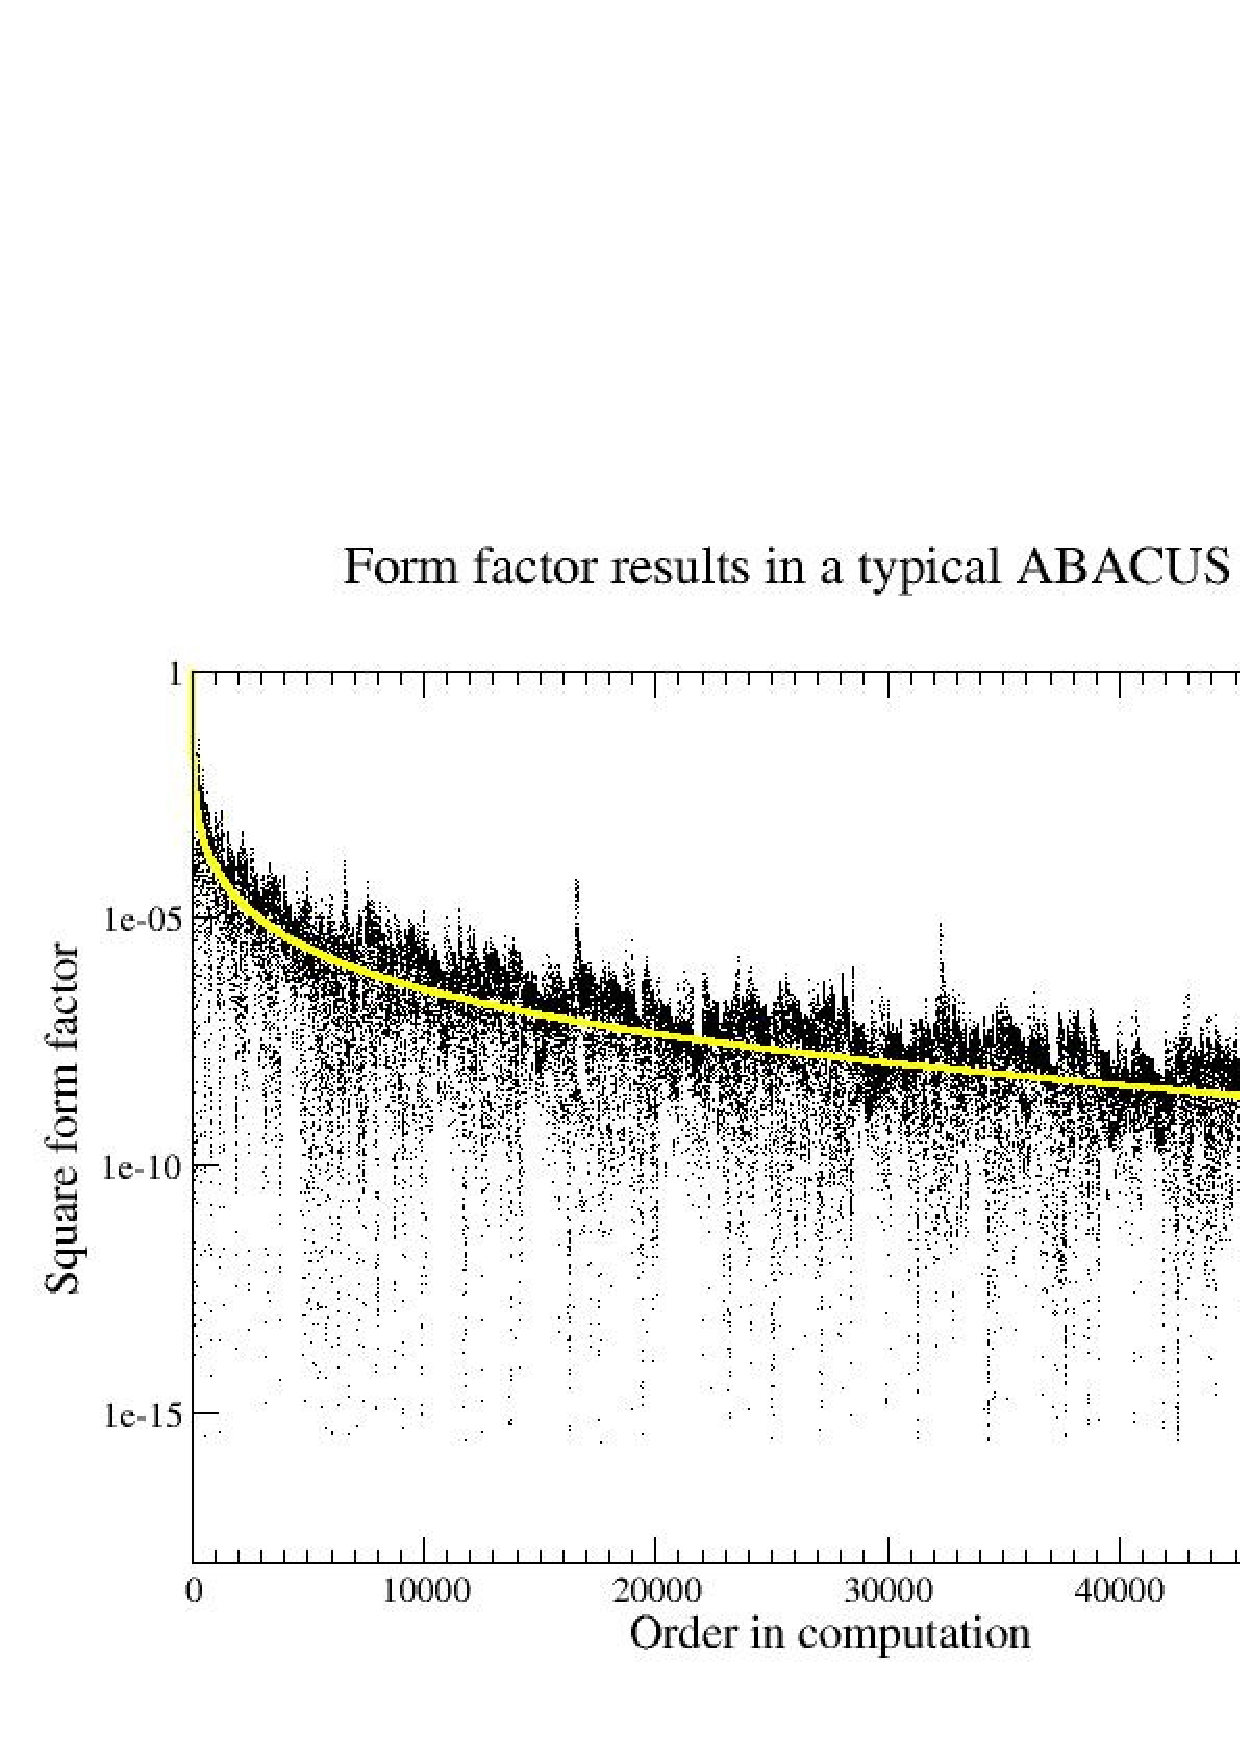
\includegraphics[width=\textwidth]{FFsq_vs_order_D0p6N50M20_small}
  \caption{Size of matrix element magnitudes encountered while summing intermediate states. The yellow line denotes strictly decreasing magnited. Note that while in general the size of the form factors decreases, not all large form factors are immediatly found. Figure taken from \cite{Caux2009}.}
\end{figure}

\begin{verbatim}
* General remarks

At the start of a simulation we choose the \alpha' to be close to \alpha.
We then scan over all states in the Hilbert space.
If states are very different, the matrix element will be small.

To scan over the Hilbert space we use the concept of a descendant.
Lets say that the matrix element <\alpha'|O\bar{O}|\alpha> ~ 10^{-2} is the largest one.
We then consider all the states adjacent to this state which have a matrix element above the scan threshold. 
The goal is to descent the "mountain" as slowly as possible. A depth first search is performed from the initial state until the threshold is crossed.
Once no more states are above the threshold, it is lowered.
In principle you will reach the entire Hilbert space in this way (though note, the Lieb-Liniger model has an infinite dimensional one).

To keep track of which states have been visited we define a thread. A thread is a line of descendents in the Hilbert space. This informaiton needs to be saved during the simulation and is saved in ".thr" files.

Note that the contributions of matrix elements are not monotonically decreasing, but may increase at some points.

The building of states happens from the outide in. The first particles are the ones that may travel the farthest in pseudo-momentum space. 
To make states unique, particles may not cross each other.
For holes the idea is the opposite.

The Bethe numbers (the Is in the Bethe equations) are multiplied by 2 to get whole numbers
This gives a vector of integers. 

Sum rules allows checking the validity of the simulation.
The contribution of states to sum rules is stored in ".src" files.
Actual summing happens in the ".sum" file.

* src/SCAN/General_Scan.cc
Contains the functions to scan over the intermediate states that are needed in the Lehmann representation to calculate Density Structure Functions.

*** Scan_LiebLin()

An initial state for the Hilbert space scan is defined: "SeedScanState".
It's the saddle point state for the partition function and density-density;
the sps with a particle in the center removed for the one-body function and the sps with a center particle added for the Green's function.


* General_Scan()
Set_Free_lambdaocs() set lambdaocs to PI * Ix2/(c * L) for (c * L) >= 1.0 and PI * Ix2/sqrt(c * L) otherwise.

\end{verbatim}

\chapter{Machine learning in the ABACUS algorithm}\label{chap:machine_learning}

\epigraph{\itshape Real stupidity beats artificial intelligence every time.}{Terry Pratchett, Hogfather}

\section{Machine learing in physics}

In the past decade machine learning has emerged as an important tool in many areas.
The increase in computing power for both CPUs and GPUs (useful for parallel linear algebra often used in machine learning) has led to a boom in research on both the commerical and academic side.
Some of the more high profile examples of this are self-driving cars (being developed by many technology and car companies) \todo{Cite this somehow?} and the development of AlphaGo, which beat the world champion in the Japanes boardgame of Go by learning from both human professional games and playing against itself \cite{Silver2017a,Silver2017}.
In the life sciences machine learning uses include detecting risk factors for cardivasular diseases from pictures of the retina \cite{poplin17_predic_cardiov_risk_factor_from} and recognizing genome variants in sequencing (with better performance than hand crafted sequencers) \cite{Poplin2016}.
Image manipulation is also benefitting from machine learning, with the ability to change the weather in pictures or transfer the species of animal in one picture to that in another \cite{Liu2017}.\footnote{What the implications are of this brave new world where no image can be fully trusted is a discussion that is only just beginning.}

In physics applications have also been found in a variety of fields.
CERN is exploring ways of tagging particles in LHC collisions using deep learning \cite{paganini17_machin_learn_algor_jet_taggin}.
In astronomy machine learning is used to classify objects in images and determine redshifts, which have to be automated due to the often large data sets resulting from even a single night of observations \cite{ball10_data_minin_and_machin_learn_in_astron}.

Condensed matter physics is now also benefitting from this field.
Recently, Carleo and Troyer~\cite{Carleo2017} proposed a way to find the ground state wavefunction of various spin systems by approximatly encoding the state of a system in a neural network. This allows for accurate approximations of the ground state energy while avoiding the exponential number of parameters encountered when representing the Hilbert space.
This technique has been extended to different systems such as the Hubbard model \cite{Saito2017}.
Phase transitions and order parameters have also been succesfully extracted from both static and periodically driven systems, using only measurable quantities such as the magnetization of individual spins \cite{Nieuwenburg2017}.

Reinforcement learning has been used to design setups for optical experiments in which complex entangled states are needed.
Since the setups are often difficult to design, reinforcement learning is used, where the computer receives a reward if an `interesting' state is created \cite{dunjko17_machin_learn_artif_intel_quant_domain}.

There are also interesting links between deep learning and physics on a more fundamental level.
For example, an exact mapping was established between the variational renormalization group en deep learning, implying that deep learning works by extracting relevant data features in a similair way to the renormalization group \cite{Mehta2014}. 

In the rest of this chapter we will review some aspects of machine learning useful in the ABACUS algorithm.\footnote{Note that we always talk here about applying machine learning to quantum mechanics, not about machine learning on quantum computers (see \cite{Dunjko2017} for that).}


\section{Machine learning: the basics}
In many cases we would like to find patterns in data.
The 

usefull for getting better initial guesses for rapidities!\todo{Really include this, it's still interesting.}
Integrate with the reinforcement learning, to get the training data. Try different neural net architectures.
\subsection{Neural networks}
Stochastic gradient descent
training, validation, testing
\subsubsection{Feedforward}
\subsubsection{Recurrent}
\subsubsection{Convolutional}



\section{Reinforcement learning}

The machine learning techniques we have described until now all rely on large data sets to function, being supervised algorithms.
They use expert data to train and this (hopefully) allows for generalization to new data.\footnote{Unsupervised algorithms that do not map an input to an output exist and are widely used, but are more suitable for tasks such as clusturing.}
In many cases however the acquisation of expert data is difficult or impossible.
In these cases reinforcement learning comes into play.
Here, there is no a priori knowledge of the targets, only a reward function that, given a state and an action returns a reward.

Have go like learning of appropriate states by considering a given state and determinging whether it is a good "close" state.
This requires some way to determine the value of a "move", a move being a mutation of a given vector of Bethe numbers\cite{Silver2017}

\subsection{Q-learning}

\subsubsection{Deep Q-networks}

interesting\cite{mnih13_playin_atari_with_deep_reinf_learn,lillicrap15_contin_contr_with_deep_reinf_learn}

\subsubsection{Recurrent Q learning}
\cite{hausknecht15_deep_recur_q_learn_partial_obser_mdps}
\subsubsection{Double Q-learning}
\cite{hasselt15_deep_reinf_learn_with_doubl_q_learn}

This fucking thing is non-Markovian, does it even make sense then?

Note however that we are working with a non-Markovian problem.
The Lieb-Liniger model itself is certainly Markovian, but the summation over states in the dynamical structure function is not, since states may not be doubly counted.
Is this still valid?
I don't know, I'm not a mathmatician, but hopefully it works.

Lets just try it and see what happens, chaning only the action selection to disallow repeat states.

Does this mostly have to do with the proofs of convergence just becoming easier when considering Markovian problems?\todo{Find out!}

\subsection{Q-learning with experience replay}

\subsection{Monte Carlo tree search}






\chapter{Methods and results}\label{chap:results}

What we are in general interested in is that, given a starting point in state space (usually the ground state), we want to explore the state space in the most efficient way possible, meaning we first visit those states in state space which have a large matrix element. 
These contribute the most to the sum in the Lehman series representation of the dynamic strucutre function.

The dimensionality of the state space for the Lieb-Liniger model (where all rapidities are real, and for a particle preserving operator) is the number of allowable choices of qunatum numbers.
If we have $M$ particles and a UV cutoff for the upper, respectively lower bound of the quantum number $I_{\infty+}$, $I_{\infty-}$, the number of states is \cite{Caux2009}\todo{Is there a symmetry factor of 1/M here?}
\begin{equation}
  I_{\infty+} + I_{\infty-} + 1 \choose M.
\end{equation}

Now we wish to define a new method to scan through the Hilbert space.
Currently a 600 line function in ABACUS does this using heuristic methods, but this function is difficult to understnad and verify.
Machine learning may offer a new way of doing this scanning.

Tge idea is to branch out from the hround state to all allowed states recursively.
The matric alements of the end poirnt of the graph thus generated are sestimated using a neural net: $NN(\{I\}) = \expval{\{\mu\}}{\mathcal{O}}{\{\lambda\}}$.
The endpoint with the largest matrix element is selected, but all the otheres are stored since they may be useful lateter.
The number of end points in the graph grows like $O(N)$ fir every iteration, so this allows us to evalute only $O(N)$ guesses per iteration.
For the selected nodes the rapidities and matrix elements are calculated to machine precision.
Then the children of this node are determind and their approximate matrix elements
Repeat until timeout or obtained sumrule is large enoug.

To compare against ABACUS we can use 2 metrics:
time used to get to a certain sumrule percentage and number of states (or percentage of Hilbert space) visited.

The guess for the matrix elements may be done with a convolutional neural network.
We treat the Behten umbers as a !D image over which we convolve.
This may also allow for transfer learning ins size since the convolution -> max pooling step downsampled



As an initial step, before exploring the intermediate state space, we create a neural network that predicts the \textit{best} or \textit{closest} state to a given base state.
In this respect we follow the approach of the Deepmind team, which first based AlphaGo on expert data and only later used tabula rase reinforcement learning.

We create a `expert' dataset by generating 10000 states represented in Bethe number space for $N=10$.
To constrain the required computation we implement a UV-cutoff in Bethe number space, with $\lvert I_{\max}\rvert=15$.\footnote{Note that, since $N$ is even, the effective maximum is $\lvert I_{\max}\rvert=14.5$.}
Every possible legal state \textit{close} to this state was than generated, where closest meant that a state has a single change in a Bethe number, with size $\Delta I = 1$.
For every adjacent state the matrix element for X\todo{Select an operator.} is calculated.
The adjacent state associated with the largest matrix element was then selected as the target state in the dataset.

Predicting the best next state is done by using two convolutional neural networks. \todo{Expand on the architecture.}
One convolutional net predicts the best place to take a Bethe number from, while the other predicts the best place to deposite the particle.


We use two approaches, one in which the tree of possible adjecent states is evaluated and traversed, and one in which only the predictions of the neural net are used for evaluation.

Simple neural net


Convolutional neural net
Pooling or no pooling (zero padding) 
Impact of data normalization on performance


Rapidities are not sensitive to the absolute size of the bethe numbers (addititive scale invariance), only their relative structure.
Therefore a vector encoding only the changed rapidities should in principle be enough to get the delta lambdas.


TWO approaches: either maximize sumrule given an set number of states or minimize number of states to achieve given sumrule


If a move is illegal the probability is set to zero and the probabilities are renormalized~\cite{pmlr-v37-clark15}.
Illegal moves are those that try to remove a particle from a position where there is none, or placing a particle on an already occupied position.
Also illegal are those moves that place particles too far away from other particles \todo{Is this necessary? Maybe it is intereseting to see what the neural net does on its own, since maybe it will come up with good states based on the training set anyway.}

verification with f-sum rule \cite{Caux2007a}
\begin{equation}
    \int \frac{\dd \omega}{2\pi} \omega S(k, \omega) = \frac{N}{L} k^2
\end{equation}

static correlator \cite{Nardis2016}
\begin{equation}
  S(k) = \int_{-\infty}^{\infty}\frac{\dd \omega}{2\pi}S(k,\omega)
\end{equation}


sumrule for one-body correlation function \cite{Caux2007}
\begin{equation}
  \frac{1}{2\pi L} \int_{\infty}^{\infty}\sum_k G_2(k,\omega) = n
\end{equation}

\section{Possible NN options}

tree like descent: given the previiusly visted states, use a nerual network to pick the best jumping off point, and another network to pick the best moves

pro: similair to how ABACUS works now, allwoing for non connected jumps through state space

con: - number of states to pick from grows linealy in time, making it difficult to choose a state (but maybe mitagetd by simply entering each state into the network separatly and then picking the one with the highest fitness)

- messy/complicated: two seperate networks

simple excitation change (used in tree like descent): a singel particle position is changed
con: only ``connected'' states may be visited in each iteration: you can only continue from the latest state
\\
full state prediction: full predict the next state given the prvious state by picking N highst ranked position from a probability distribution

pro:smaller output space

con: unclear what to do with already visited states
\\
Add penalty in reward function for every visited state?
\\
ideas:
use convolution over history of states

use convulution over state

reward may be either immediate or delayed

\section{A neural net for each no of ph pairs}
Maybe there should be multple neural nets, one for each possible number of ph-pairs (up to a certain max number).
So you would first try 1 ph, than 2, etc...

\section{The Lieb-Liniger ``game''}

To stay in the spirit of the results of Deepmind we will cast the stepping through the state-space of the Lieb-Liniger model in the form of a game with certain rules.
The rules are:
\begin{itemize}
  \item no moves that lead to an already visited state
  \item able to reach all states in the given momentum interval
  \item sample important states first
\end{itemize}

The maximum momentum $I_{max}$ is for the total momentum of the state, not the individual components, (so some particles can have high momentum, if it is compensated for by another particle with opposite negative momentum.)

A possible way to quickly determine large MEs is to simplify the matrix element calculations by considering only the diagonal and first off-diagonals, which are then of the order $\frac{1}{(\mu-lambda)^2 + 1/L^2}$

ABACUS can scan within an idividual slice.
What you got may work for the partition function, where only energies matter, since those are not spanning so many orders of magnitude.

The number of possible 1 ph-pair states increase with k up to a certain k and then saturates at a level of order $N$.
For 2 ph-pairs it saturatiates at $N^3$

We use the neural net to tell us which move to make.
To that end we use the same representation of moves as Alpha Zero uses in chess \cite{Silver2017}, except ``playing'' on a one dimensional board instead of a two dimensional chess board.
Available moves can be represented as a tuple, with the x-coordinate representing the location of the particle to remove and the y-coordiate being the new coordinate on which the particle is placed.
This is represented by an $N_{sites} \times N_{sites}$ matrix, with the value of each matrix element coming from the neural net used for Q-learning.

We represent state as vectors with lenght $N_{sites} = 2 I_{max} + 1$.
Particles are denoted with 1's, and all other entries are zero.
For example, the ground state of the $N=3$ state with $I_{max} = 5$ is 
\begin{equation}
  \begin{pmatrix} 0 & 0 & 0 & 0 & 1 & 1 & 1 & 0 & 0 & 0 & 0 \end{pmatrix}
\end{equation}

Note that the learning is all tabula rase reinforcement learning

\section{Exact saturation results}

Exact results of saturations in small systems.

\section{The f-sum rule}
To verify that we have summed form factors that contribute a lot to the density structure function, we can use the f-sum rule.

\section{Results}

If $c = n  x$ and $L = y$, than the ideal ordening of matrix elements for this setup translates to the case where $c = x$ and $L = n y$, for $n \in \mathbb{R}$.
In other words, making the interaction strength $n$ times larger maps to the same system in matrix element ordering space as make the system size $n$ times smaller.

If one of the parameters is perturbed by a factor $1+k$ with $k$ small, than the difference between the matrix elements is of order $k$.

In general matrix elements for the different parameter families mentioned above differ only by a factor $n$, meaning that you can calculate the matrix elements for the different systems by a simple rescaling.

Conjecture: The ordering of matrix elements is the same as long as the parameter $\gamma$ is the same. The value of the matrix elements is the same up to the factor with which the lenght of the system has been scaled.

PROBLEM: We never reward in the experience replay because we never reach a terminal state. The reward function has to be edited to take this into account.

\subsection{Random action selection}

\subsection{Q-learning}

\subsection{Q-learning with memory replay}

\subsection{Verification}


\subsection{Machine learning rapidities and operator matrix elements}

\chapter{Discussion and conclusion}\label{chap:conclusion}

\epigraph{\itshape I may not have gone where I intended to go, but I think I have ended up where I needed to be.}{Douglas Adams, The Long Dark Tea-Time of the Soul}


Transfer learning ay be used to generalize from different states.

Inadmissable states may be ignored.

As mentioned in \cite{Caux2009} the applicability of ABACUS for large systems stems from the preliminary information provided by integrability, built into the algorithm.

AI is creative \cite{1803.03453}.

Better averaging state: high entropy state as averaging state because that makes the matrix element space flatter in sizes

In general reinforcement learning is very data inefficient, leading to the conejcture that a well crafted function may work better in this domain \cite{1710.02298}.

Reproducibility of RL solutions is often an issue \cite{1709.06560}.

\appendix


\chapter{The f-sum rule}

When computing the dynamical structure function numerically we need a way to measure what fraction of relevant states have been summed.
To that end we can use the f-sum rule, which is a model-independent equality linking an integral over the dynamic structure function to a commutator of the Hamiltonian of the system and the operator under investigation \cite{pitaevskii}.
We first derive the general formula and then find sum rules for specific operators.


In general we are interested in the correlation function of an operator $\mathcal{O}$:
\begin{align}
  \expval{\mathcal{O}_j^a(t)\mathcal{O}_{j'}^{\bar{a}}(0)},
\end{align}
where $j, j'$ are arbitrary points on a lattice, we consider arbitrary time differences $t$, $a$ is a label denoting the operator and

\todo{Also known as Thomas-Reich-Kuhn sumrule \cite{pitaevskii}}

Sum rule factors in ABACUS: used in saturation calculation, you can also just use LHS/RHS

\section{The $\rho$ operator}

The operator is $\expval{\{\mu\}}{\rho(x=0)}{\{\lambda\}}$, where $\rho(x=0) = \frac{1}{L} \sum{k''} e^{-i k'' x} \rho_{k''} |_{x=0}$ 

\section{The $:\rho^2:$ operator}

The $:\rho^2:$ operator is equal to  $(\psi^{\dagger})^2\psi^2$

\chapter{LU decomposition}\label{app:ludecomp}


\bibliographystyle{SciPost_bibstyle}
\bibliography{master_thesis_references}



\end{document}
